\section{Implementation, integration and test plan}

    
    We now want to present how we will implement our system by explaining the strategy we will follow for the Server
    and how the features we want to offer will be implement and integrated.\\
        
        \subsection{Server}
        The Server will be implemented following a bottom-up strategy since it will be built on various modules that will cooperate in order
        to ensure that the goals and standards stated in the \emph{RASD}\cite{RASD} will be met.\\
        The Server relies on the GIS and the Municipality API, which will be considered reliable and accurate services and will be
        tested only "server side" (i.d. checking that our system can exploit them properly).\\
        For what it concerns the the Server, each submodule will be implemented and tested with formal methods before being integrated 
        with the other modules that rely on it, since integrating a malfunctioning module with other can only lead to bigger problems 
        and the effort and time needed to fix them could increase exponentially.\\
        To better understand the decisions we made about implementation, testing and integration here are two tables that list the features
        we want to offer linked with the relevance we gave them considering the difficulty of the implementation and the importance for 
        the user.\\
        
        \subsection{UserApplication features}
        \begin{table}[h!]
            \begin{center}
            
            \begin{tabular}{l|c|r} % <-- Alignments: 1st column left, 2nd middle and 3rd right, with vertical lines in between
                \textbf{Feature} & \textbf{Importance} & \textbf{Difficulty of implementation}\\
                
                \hline
                Sign up and login & Low & Low\\
                Consult personal data & Low & Low\\
                Upload a picture & High & Medium\\
                Consult the map & Medium & High\\
                See statistics & Medium & High\\

            \end{tabular}
            \caption{Users features}
            \label{tab:table1}
            \end{center}
        \end{table}

        \begin{itemize}
            \item \textbf{Sign up and login:} sign up and login are features that are fundamental to identify users and allow them to 
                properly upload reports. The modules that will support the login phase will be \emph{AccessHandler}, that will be 
                implemented right before the \emph{UserInformationHandler} since their functionalities are linked. Moreover they 
                will be tested following the "relies on" relationship. They both rely on \emph{DataProvider} module, so their testing 
                procedure will be subjected to the one of the \emph{DataProvider} and the same stands for the integration procedure
            \item \textbf{Consult personal data:} the module \emph{UserInformationHandler} is the one responsible of making this feature 
                available. It will be integrated with the \emph{DataProvider}, and will be implemtented after the \emph{AccessHandler} since
                a user needs to sign up to the system before accessing his information
            \item \textbf{Upload a picture:} this feature is the core of the whole system, and several modules are involved in its 
                realization. The \emph{SubmissionHandler} is responsible of coordinating all the operations and method calls necessary 
                to perform the action. It will call the \emph{DataProvider} and will interact with the \emph{GIS}, for these reasons it
                will be integrated with them.
            \item \textbf{Consult the map:} this feature will concerne the \emph{DataProvider}, the \emph{MapHandler} and the 
                \emph{GIS API}. The first one will be responsible of retrieving the proper information from the database, 
                while the \emph{MapHandler} will format the data sent from the \emph{userAppServer} in order to forward it to the 
                \emph{GIS API} to allow it to offer the rendered map
            \item \textbf{See statistics:} the \emph{StatisticsHandler} will trigger the \emph{DataProvider} to retrieve updated
                data from the \emph{Municipality API} and the \emph{DBMS} with the objective of updating all the possible 
                statistics that the system will offer to the user and the Municipality
        \end{itemize}
       
        \subsection{Municipality features}
        \begin{table}[h!]
            \begin{center}
            
            \begin{tabular}{l|c|r} % <-- Alignments: 1st column left, 2nd middle and 3rd right, with vertical lines in between
                \textbf{Feature} & \textbf{Importance} & \textbf{Difficulty of implementation}\\
                
                \hline
                Authenticate & Low & Low\\
                Access the API & High & Low\\
                Retrieve violations' data & High & Medium\\
                Retrieve statistics & Medium & Medium\\
                Retrieve tickets's data & High & High\\
                Share data & Medium & Medium\\

            \end{tabular}
            \caption{Municipality features}
            \label{tab:table1}
            \end{center}
        \end{table}

        All these features will be made available through the \emph{API}. Since it will be of fundamental importance for the 
        system's interface with the Municipality it will have to be implemented on a strong and reliable backend (all the 
        "logic" modules) and for this reason it will be implemented after the whole Server will be fully tested.\\

    \subsection{Integration}

        In this section we want to show how we want to integrate modules with one another. The tail of the arrow starts from the module 
        that uses the one pointed by the head.\\
        Even with the most rigorous testing procedure the integration can generate unpredictable side effects, so right after two modules 
        are integrated they are tested again, and so on until the whole Server of the system will be fully implemented.

        \subsubsection{Integration of the internal components of the Server}
            
            For better readability we separated the pictures of the integration of the \emph{DataProvider} with the other modules of the backend.\\

            \begin{figure}[h]
                \centering
                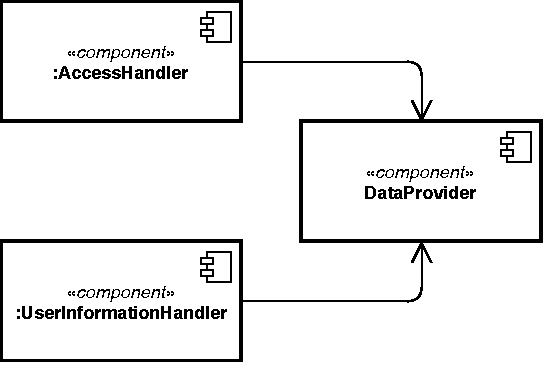
\includegraphics[width=0.5\linewidth]{userDataIntegration}
                \caption{
                    \label{fig:userDataIntegration} 
                    User data integration
                }
            \end{figure}
            
            \begin{figure}[h]
                \centering
                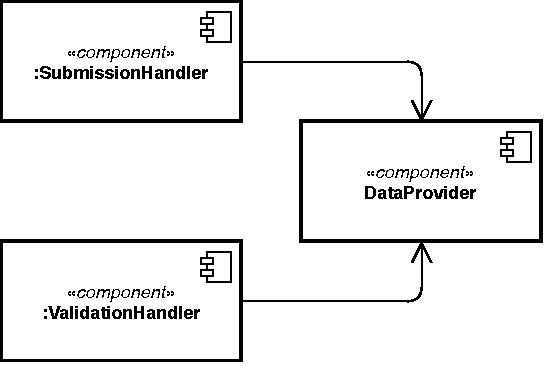
\includegraphics[width=0.5\linewidth]{submissionDataIntegration}
                \caption{
                    \label{fig:submissionDataIntegration} 
                    Submissions and violations data integration
                }
            \end{figure}
            
            \begin{figure}[h]
                \centering
                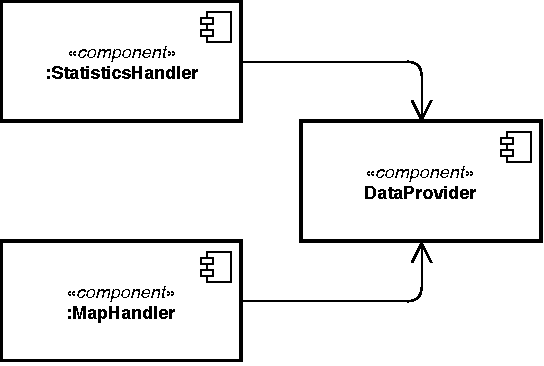
\includegraphics[width=0.5\linewidth]{statisticsDataintegration}
                \caption{
                    \label{fig:statisticsDataIntegration} 
                    Statistics and map data integration
                }
            \end{figure}
             
            \begin{figure}[h]
                \centering
                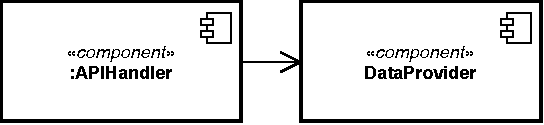
\includegraphics[width=0.5\linewidth]{apiDataIntegration}
                \caption{
                    \label{fig:apiDataIntegration} 
                    Municipality API data integration
                }
            \end{figure}
            \clearpage

        \subsubsection{Integration of the frontend with the backend}
            
            The \emph{UserApplication} and the \emph{CustomerCareApplication} are considered to be frontend modules 
            since they are the connection with the external world. These modules will be the last to be integrated because, 
            as already stated, we want to be sure to expose well implemented interfaces before doing so.\\

            \begin{figure}[h]
                \centering
                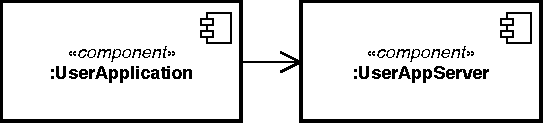
\includegraphics[width=0.5\linewidth]{userAppIntegration}
                \caption{
                    \label{fig:userAppIntegration} 
                    User app integration
                }
            \end{figure}
             
            \begin{figure}[h]
                \centering
                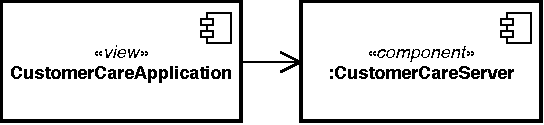
\includegraphics[width=0.5\linewidth]{customerCareIntegration}
                \caption{
                    \label{fig:customerCareIntegration} 
                    Customer Care integration
                }
            \end{figure}

        \subsubsection{Integration with the external services}
            
            The \emph{GIS} and the \emph{Municipality} are the external services with which our sistem interfaces, and will be
            integrated at different stages of implementation.\\
            The \emph{GIS} will be integrated with the \emph{:MapHandler} component since the latter relies on it, 
            while the \emph{Municipality API} will be integrated as soon as the backend will be properly implemented.


        


